%\documentclass[aspectratio=43]{beamer}
\documentclass[t]{beamer}
\usetheme{ffmodernnopagenum}  %% Themenwahl

\usepackage[ngerman]{babel} 
\usepackage[T1]{fontenc}    % richtige Silbentrennung
\usepackage[utf8]{inputenc} % Umlaute etc.!
\usepackage{eurosym}
\usepackage{tikz}
\usepackage{pgffor}
\usepackage[absolute,overlay]{textpos}
\usepackage[document]{ragged2e}

\usetikzlibrary{arrows,decorations.pathmorphing,backgrounds,fit,positioning,shapes.symbols,chains}

\title{Freifunk Hamburg}
\author{Andreas Baldeau}
\date{23. September 2015}
\license{CC-BY-3.0}

\begin{document}
\maketitle

\begin{frame}{}
    \vspace{3.4cm}
    \centering \Huge\bf Freifunk\hl{?}
\end{frame}

\begin{frame}{}
    \begin{textblock*}{8.8cm}(2.8cm,3.2cm)
        \Large\bf
        „Freifunk ist eine nicht\-kommerzielle \\
        Initiative, die sich dem Aufbau und \\
        Betrieb eines freien Funknetzes, das \\
        aus selbstverwalteten lokalen \\
        Computer\-netzwerken besteht, \\
        widmet.“
    \end{textblock*}

    \vspace{7cm}
    \hspace{4.1cm}
    {\scriptsize(Wikipedia-Artikel „Freifunk“, Stand 24. August 2015)}
\end{frame}



%%% Initiative %%%%%%%%%%%%%%%%%%%%%%%%%%%%%%%%%%%%%%%%%%%%%%%%%%%%%%%%%%%%%%%%

\begin{frame}{}
    \begin{textblock*}{8.8cm}(2.8cm,3.13cm)
        \Large\bf
        „Freifunk ist eine \hl{\LARGE nicht\-kommerzielle} \\
        \hl{\LARGE Initiative}, die sich dem Aufbau und \\
        Betrieb eines freien Funknetzes, das \\
        aus selbstverwalteten lokalen \\
        Computer\-netzwerken besteht, \\
        widmet.“
    \end{textblock*}

    \vspace{7cm}
    \hspace{4.1cm}
    {\scriptsize(Wikipedia-Artikel „Freifunk“, Stand 24. August 2015)}
\end{frame}

\begin{frame}{}
    \begin{center}
        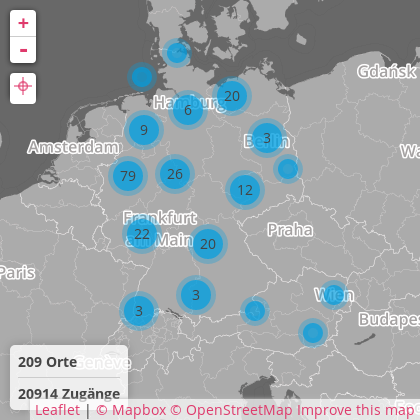
\includegraphics[width=.7\textwidth]{Bilder/community-map-2015-09-22}
    \end{center}
\end{frame}



%%% Aufbau %%%%%%%%%%%%%%%%%%%%%%%%%%%%%%%%%%%%%%%%%%%%%%%%%%%%%%%%%%%%%%%%%%%%

\begin{frame}{}
    \begin{textblock*}{9.2cm}(2.8cm,3.2cm)
        \Large\bf
        „Freifunk ist eine nicht\-kommerzielle \\
        Initiative, die sich dem \hl{\LARGE Aufbau und} \\
        \hl{\LARGE Betrieb} eines freien Funknetzes, das \\
        aus selbstverwalteten lokalen \\
        Computer\-netzwerken besteht, \\
        widmet.“
    \end{textblock*}

    \vspace{7cm}
    \hspace{4.1cm}
    {\scriptsize(Wikipedia-Artikel „Freifunk“, Stand 24. August 2015)}
\end{frame}

\begin{frame}{}
    \begin{center}
        \includegraphics[width=.6\textwidth]{Bilder/fux-klettern}
    \end{center}
\end{frame}



%%% frei %%%%%%%%%%%%%%%%%%%%%%%%%%%%%%%%%%%%%%%%%%%%%%%%%%%%%%%%%%%%%%%%%%%%%%

\begin{frame}{}
    \begin{textblock*}{10cm}(2.8cm,3.2cm)
        \Large\bf
        „Freifunk ist eine nicht\-kommerzielle \\
        Initiative, die sich dem Aufbau und \\
        Betrieb eines \hl{\LARGE freien} Funknetzes, das \\
        aus selbstverwalteten lokalen \\
        Computer\-netzwerken besteht, \\
        widmet.“
    \end{textblock*}

    \vspace{7cm}
    \hspace{4.1cm}
    {\scriptsize(Wikipedia-Artikel „Freifunk“, Stand 24. August 2015)}
\end{frame}



%%% Funknetze %%%%%%%%%%%%%%%%%%%%%%%%%%%%%%%%%%%%%%%%%%%%%%%%%%%%%%%%%%%%%%%%%

\begin{frame}{}
    \begin{textblock*}{10cm}(2.8cm,3.2cm)
        \Large\bf
        „Freifunk ist eine nicht\-kommerzielle \\
        Initiative, die sich dem Aufbau und \\
        Betrieb eines freien \hl{\LARGE Funknetzes}, das \\
        aus selbstverwalteten lokalen \\
        Computer\-netzwerken besteht, \\
        widmet.“
    \end{textblock*}

    \vspace{7cm}
    \hspace{4.1cm}
    {\scriptsize(Wikipedia-Artikel „Freifunk“, Stand 24. August 2015)}
\end{frame}

\begin{frame}{}
    \begin{center}
        \includegraphics[width=1\textwidth]{Bilder/richtfunk-fux}
    \end{center}
\end{frame}

\begin{frame}{}
    \vspace{3cm}
    \begin{center}
        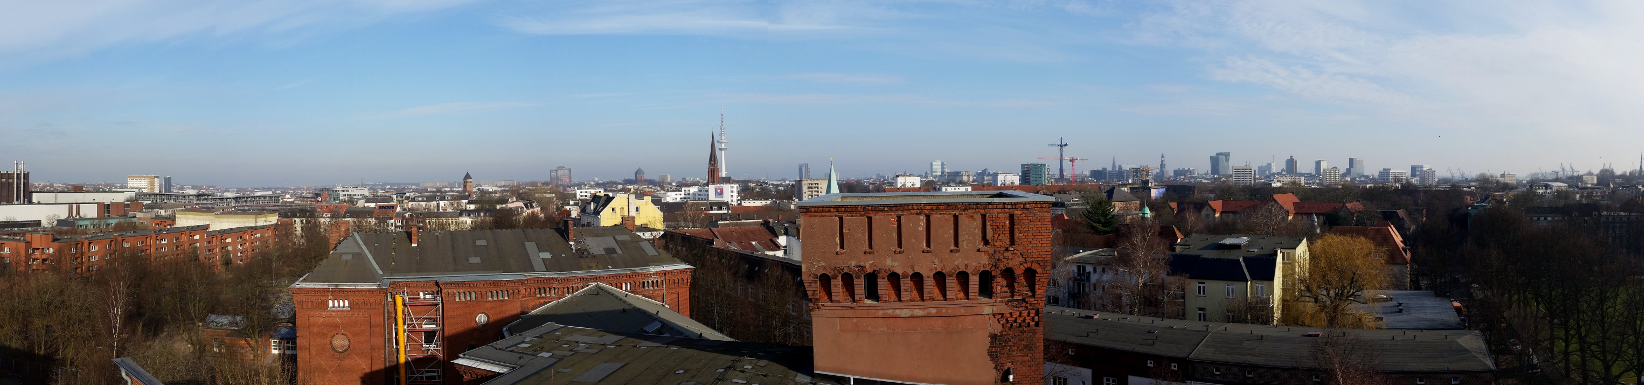
\includegraphics[width=1\textwidth]{Bilder/fux-panorama}
    \end{center}
\end{frame}

\begin{frame}{}
    \begin{center}
        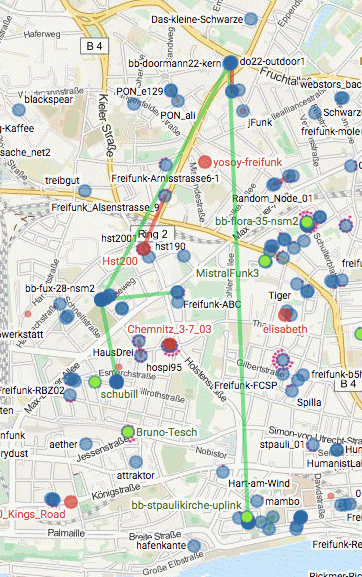
\includegraphics[width=.5\textwidth]{Bilder/backbone-2015-09-22}
    \end{center}
\end{frame}



%%% selbstverwaltet %%%%%%%%%%%%%%%%%%%%%%%%%%%%%%%%%%%%%%%%%%%%%%%%%%%%%%%%%%%

\begin{frame}{}
    \begin{textblock*}{10cm}(2.8cm,3.2cm)
        \Large\bf
        „Freifunk ist eine nicht\-kommerzielle \\
        Initiative, die sich dem Aufbau und \\
        Betrieb eines freien Funknetzes, das \\
        aus \hl{\LARGE selbstverwalteten} lokalen \\
        Computer\-netzwerken besteht, \\
        widmet.“
    \end{textblock*}

    \vspace{7cm}
    \hspace{4.1cm}
    {\scriptsize(Wikipedia-Artikel „Freifunk“, Stand 24. August 2015)}
\end{frame}

\begin{frame}{}
    \begin{center}
        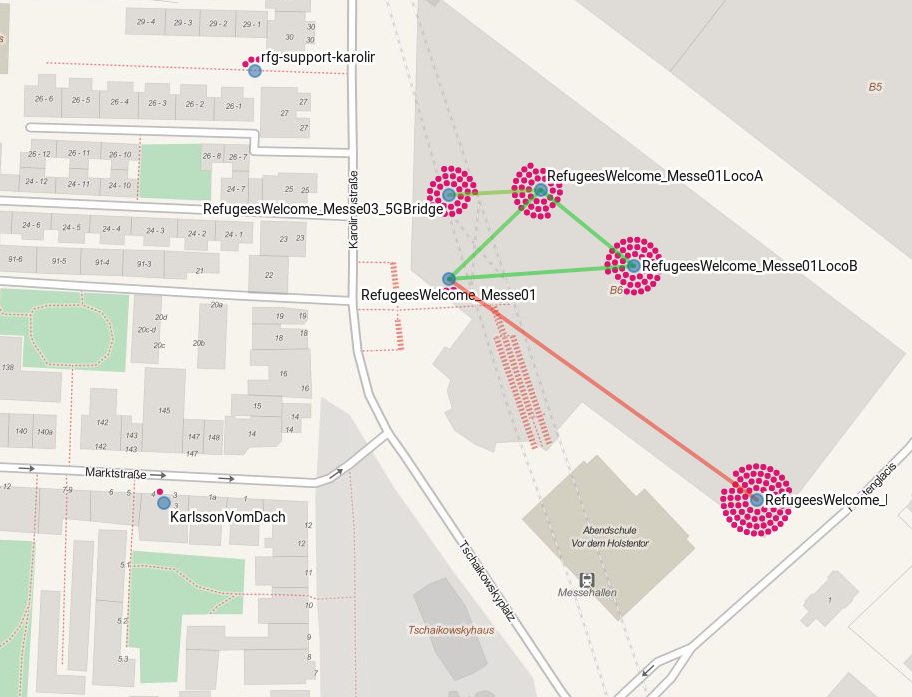
\includegraphics[width=.9\textwidth]{Bilder/messe-refugees-welcome}
    \end{center}
\end{frame}



%%% lokal %%%%%%%%%%%%%%%%%%%%%%%%%%%%%%%%%%%%%%%%%%%%%%%%%%%%%%%%%%%%%%%%%%%%%

\begin{frame}{}
    \begin{textblock*}{10cm}(2.8cm,3.2cm)
        \Large\bf
        „Freifunk ist eine nicht\-kommerzielle \\
        Initiative, die sich dem Aufbau und \\
        Betrieb eines freien Funknetzes, das \\
        aus selbstverwalteten \hl{\LARGE lokalen} \\
        Computer\-netzwerken besteht, \\
        widmet.“
    \end{textblock*}

    \vspace{7cm}
    \hspace{4.1cm}
    {\scriptsize(Wikipedia-Artikel „Freifunk“, Stand 24. August 2015)}
\end{frame}

\begin{frame}{}
    \begin{center}
        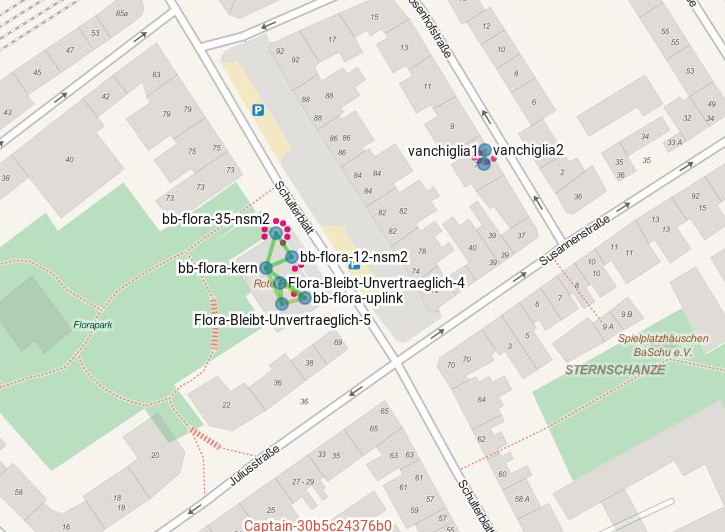
\includegraphics[width=.9\textwidth]{Bilder/flora-2015-09-22}
    \end{center}
\end{frame}

\begin{frame}{}
    \begin{center}
        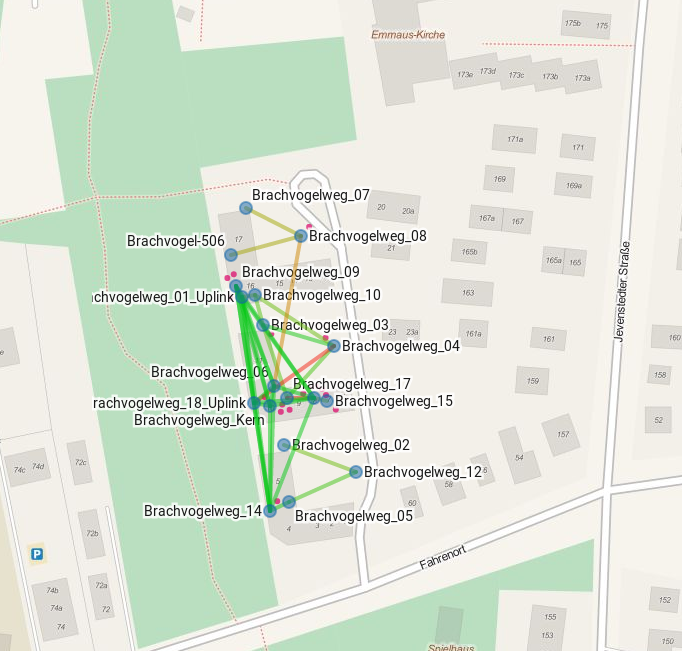
\includegraphics[width=.7\textwidth]{Bilder/brachvogel-2015-09-22}
    \end{center}
\end{frame}

\begin{frame}{}
    \begin{center}
        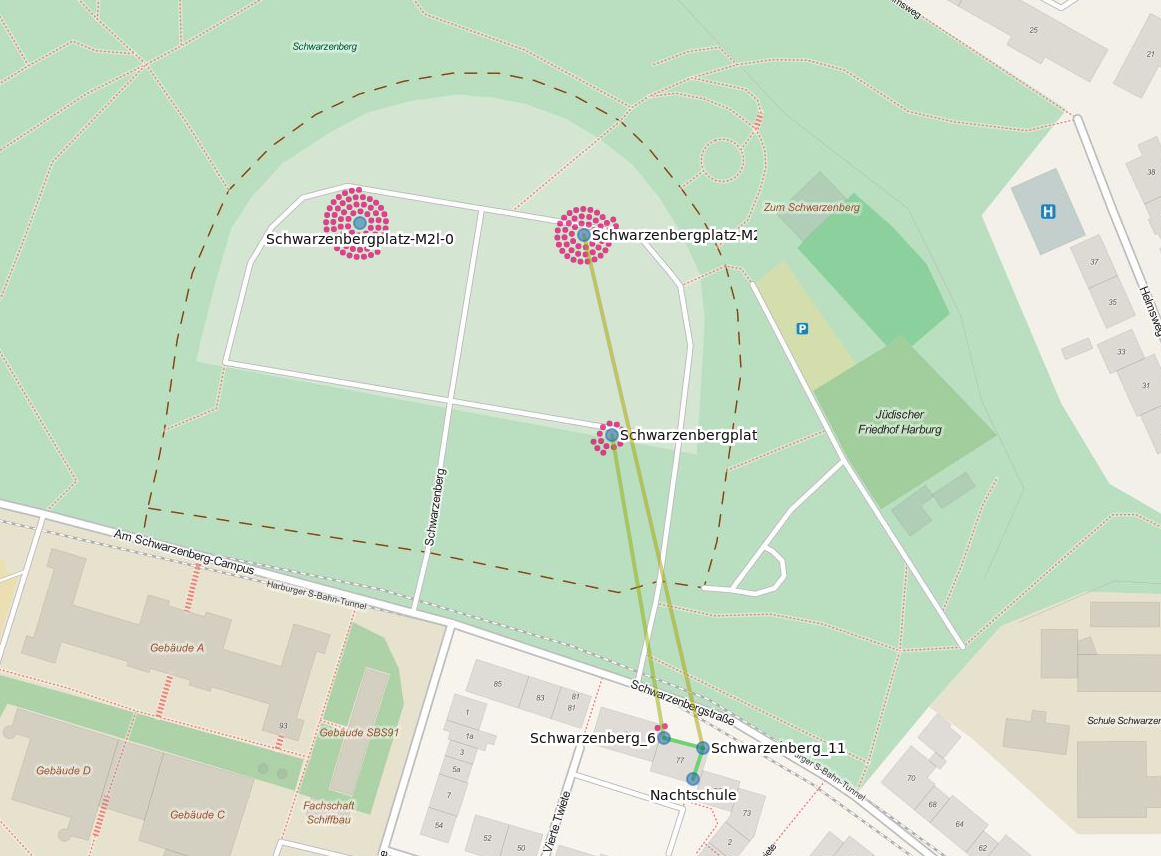
\includegraphics[width=.9\textwidth]{Bilder/schwarzenberg-2015-09-22}
    \end{center}
\end{frame}



%%% Im Hamburg funkt man frei %%%%%%%%%%%%%%%%%%%%%%%%%%%%%%%%%%%%%%%%%%%%%%%%%

\begin{frame}{}
    \vspace{3.4cm}
    \centering \Huge\bf In Hamburg\hl{...}
\end{frame}


\begin{frame}{}
    \vspace{0.6cm}
    \centering \includesvg[width=5cm]{in-hamburg-funkt-man-frei}
    \vspace{0.3cm}

    \bf 
    hamburg.freifunk.net \\
    \vspace{0.1cm}
    twitter.com/FreifunkHH -- facebook.com/FreifunkHamburg \\
    \vspace{0.1cm}
    irc://irc.hackint.net/ffhh \\
    \vspace{0.1cm}
    Montags 19:00 CCCHH, Freitags 19:30 Attraktor e. V.
\end{frame}









%%% Wie funktionierts? %%%%%%%%%%%%%%%%%%%%%%%%%%%%%%%%%%%%%%%%%%%%%%%%%%%%%%%%

\foreach \index in {1, ..., 3} 
{
    \begin{frame}{}
        \vspace{1.3cm}
        \centering \includesvg[width=9cm]{netz-\index}
    \end{frame}
}

\begin{frame}{}
    \vspace{1.3cm}
    \centering \includesvg[width=9cm]{netz-4-neu}
\end{frame}

\end{document}
